\documentclass{beamer}
\usepackage[utf8]{inputenc}
\usepackage{default}
\usepackage{hyperref}
\usepackage[czech]{babel}
\usepackage{subfigure}

\usetheme{Madrid}
\usecolortheme{seagull}

\title{Raspberry Pi}
\date{26. května 2014}
\author{Tomáš Havlík \\(havlito5@fit.cvut.cz)}

\begin{document}

\begin{frame}
\titlepage
\end{frame}

\begin{frame}\frametitle{Co to je?}
\begin{itemize}
\item jednodeskový počítač o velikosti platební karty
\item \href{http://raspberrypi.org}{Raspberry Pi Foundation}
\item podpora výuky informatiky
\end{itemize}
\begin{figure}[htp]
\centering

\includegraphics[scale=.2]{rpi_logo.png}
\end{figure}
\end{frame}

\begin{frame}\frametitle{Hardware}
\begin{itemize}
\item CPU: 700 MHz ARM
\item GPU: 250 MHz Broadcom
\item RAM: 256 / 512 MB (sdílená)
\item rozsáhlé možnosti I/O
\item 1.5 W / 3.5 W
\item \$25 (Model A) / \$35 (Model B)
\end{itemize}
\begin{figure}[htp]
\centering
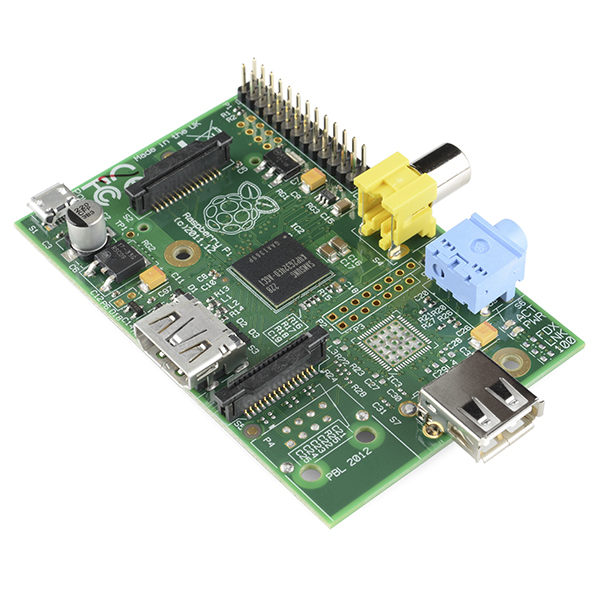
\includegraphics[scale=.3]{modA.jpg}
\end{figure}
\end{frame}

\begin{frame}\frametitle{Operační systémy}
\centering

\includegraphics[width=0.2\textwidth]{raspbian.png}

\includegraphics[width=0.2\textwidth]{pidora.png}

\includegraphics[width=0.2\textwidth]{openelec.png}\\

\includegraphics[width=0.2\textwidth]{raspbmc.png}

\includegraphics[width=0.2\textwidth]{riscos.png}

\includegraphics[width=0.2\textwidth]{arch.png}

\begin{exampleblock}{Instalace operačního systému}
\begin{enumerate}
\item stažení balíčku NOOBS
\item naformátování a flashnutí SD karty
\item výběr distribuce
\end{enumerate}
\end{exampleblock}
\end{frame}

\begin{frame}\frametitle{Způsoby využití}
\begin{enumerate}
\item programování (C++, Python, Scratch)
\item multimediální centrum
\item file server
\item ovládání hardware
\item kancelářské PC
\end{enumerate}
\begin{alertblock}{Wolfram Mathematica}
Každý vlastník má možnost stáhnout si plnou verzi aplikace Mathematica pro osobní použití.
\end{alertblock}
\end{frame}

\begin{frame}\frametitle{Ukázka}
\centering
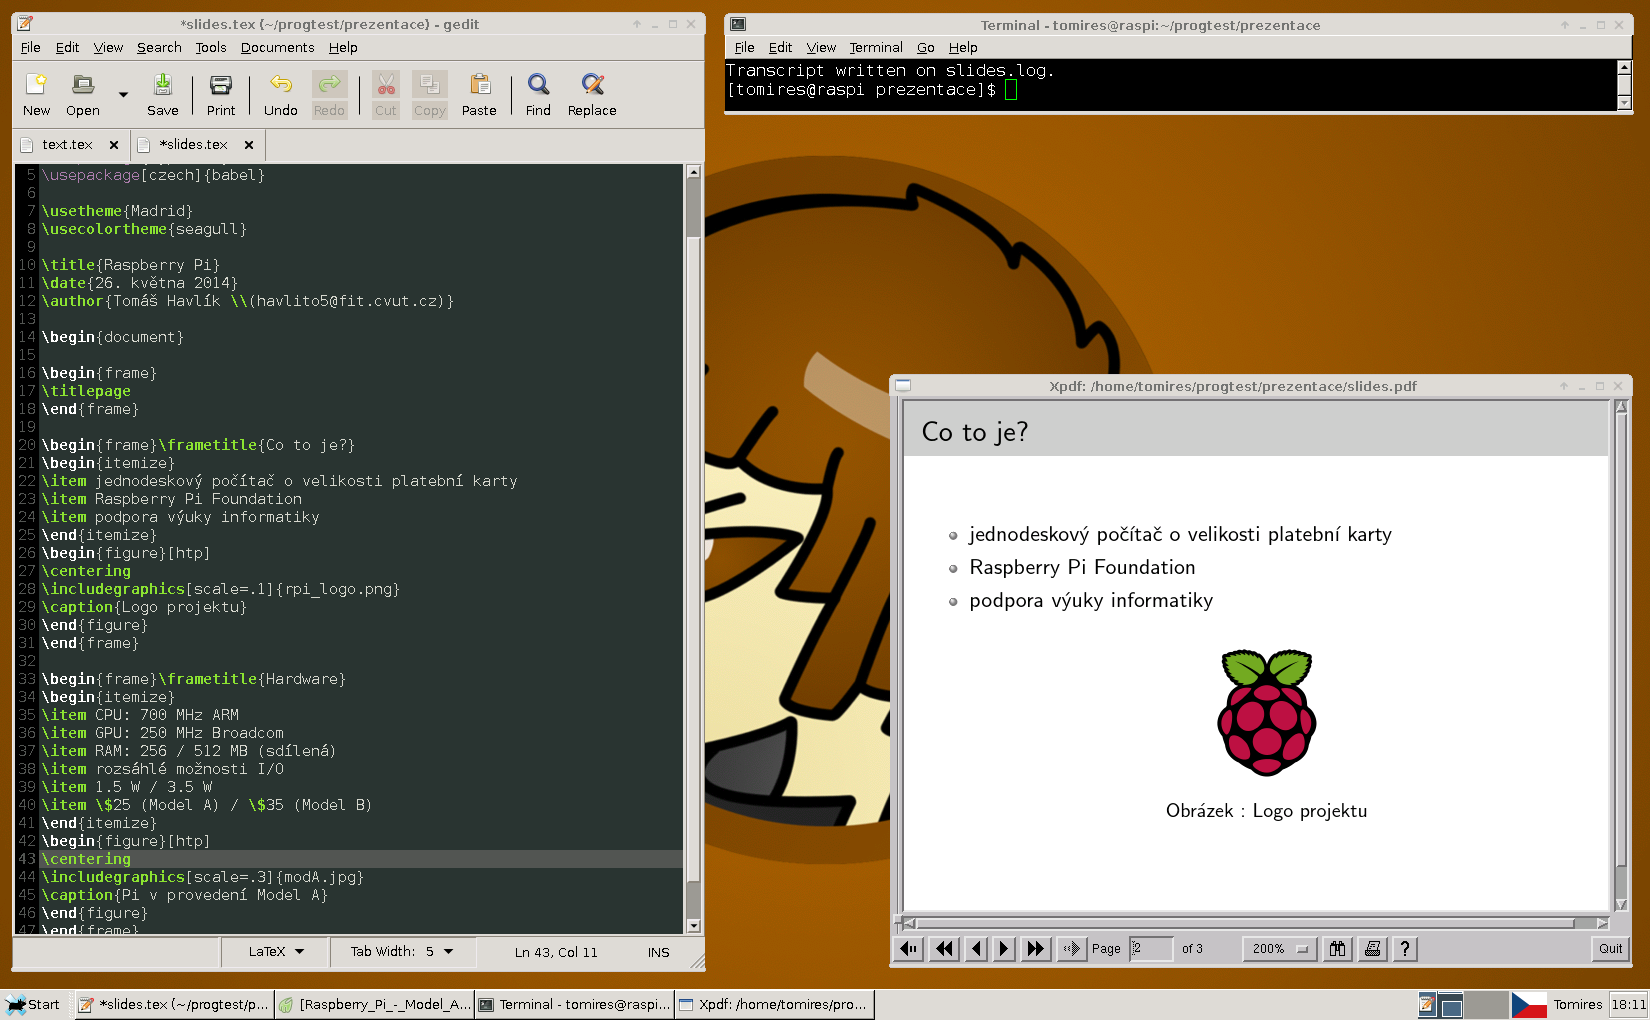
\includegraphics[keepaspectratio=true,width=0.95\paperwidth]{screen.png}
\end{frame}

\begin{frame}\frametitle{Děkuji za pozornost \^{}\_\^{}}
\centering
Více informací najdete na
\begin{itemize}
\centering
\item \href{http://raspberrypi.org}{raspberrypi.org}
\item \href{http://element14.com/community/community/raspberry-pi}{element14.com}
\item \href{http://wolfram.com/raspberry-pi}{wolfram.com}
\end{itemize}
\centering

\includegraphics[scale=.3]{android.png}
\end{frame}

\end{document}
